\chapter{Convex Hulls}
\label{ch:convex_hulls}

\section{Graham Scan}
\label{sec:graham_scan}

The Graham scan is an efficient method for computing the convex hull\index{convex hull} of a finite set of points in the Euclidean plane. It was published by Ronald Graham in 1972~\cite{graham1972} and is a fundamental algorithm in computational geometry. The algorithm finds all vertices of the convex hull ordered along its boundary.

\subsection{Definitions}

\begin{definition}[Convex Hull]\label{def:convex_hull}
The \emph{convex hull} of a set $S \subseteq \mathbb{R}^2$ is the smallest convex set containing all the points in~$S$. Equivalently, it is the intersection of all convex sets containing~$S$, or the set of all convex combinations of points in~$S$:
\[
\operatorname{conv}(S) = \left\{ \sum_{i=1}^{k} \lambda_i p_i \;\Big|\; k \in \mathbb{N},\; p_i \in S,\; \lambda_i \ge 0,\; \sum_{i=1}^{k} \lambda_i = 1 \right\}.
\]
\end{definition}

\begin{definition}[Cross Product in $\mathbb{R}^2$]\label{def:cross_product_2d}
For three points $A, B, C \in \mathbb{R}^2$, the \emph{cross product} is defined as
\[
\operatorname{cross}(A, B, C) = (B.x - A.x)(C.y - A.y) - (B.y - A.y)(C.x - A.x).
\]
It determines the orientation of the ordered triple $(A, B, C)$:
\begin{itemize}
\item Positive: Left turn (counter-clockwise).
\item Negative: Right turn (clockwise).
\item Zero: Collinear.
\end{itemize}
Geometrically, $|\operatorname{cross}(A,B,C)|$ equals twice the signed area of triangle $\triangle ABC$.
\end{definition}

\begin{definition}[Anchor Point]\label{def:anchor_point}
The \emph{anchor point} of a point set is the point with the lowest $y$-coordinate (and lowest $x$-coordinate in case of ties). It is guaranteed to lie on the convex hull.
\end{definition}

\subsection{Theory}

The algorithm operates by first identifying an extreme point (the anchor\index{anchor point}) and sorting all other points based on the polar angle they make with this anchor. It then performs a linear scan through the sorted points, maintaining a stack of points that potentially form the hull. For each new point, the algorithm ``backtracks'' by popping points from the stack that would create a non-convex (right) turn. This ensures that the final stack contains only the vertices of the convex hull in counter-clockwise order.

\begin{theorem}[Correctness of the Graham Scan]\label{thm:graham_scan_correctness}
Let $P$ be a set of $n \ge 3$ points in general position in $\mathbb{R}^2$, and let $p_0$ be the anchor point. After sorting the remaining points by polar angle around $p_0$, the Graham scan produces the vertices of $\operatorname{conv}(P)$ in counter-clockwise order.
\end{theorem}
\begin{proof}
The key invariant is that the stack always stores a sequence of points forming a left-turn chain. When a new point $p_i$ is examined, any point(s) on the stack that would create a right turn (i.e., $\operatorname{cross}(s_{k-1}, s_k, p_i) \le 0$) are removed. Since every vertex of the convex hull must appear as a left turn when traversed counter-clockwise, no hull vertex is ever popped. Conversely, every non-hull point is eventually popped because it must lie inside the convex polygon formed by the hull vertices, and hence some subsequent hull vertex will create a right turn with it. The remaining stack therefore contains exactly the hull vertices in order.
\end{proof}

\begin{theorem}[Complexity of the Graham Scan]\label{thm:graham_scan_complexity}
The Graham scan computes the convex hull of $n$ points in $O(n \log n)$ time and $O(n)$ space.
\end{theorem}
\begin{proof}
The sorting step dominates with cost $O(n \log n)$. In the scan phase, each point is pushed onto the stack exactly once. Each point is popped at most once (since once popped, it is never re-examined). Thus the total number of push and pop operations is $O(n)$, making the scan phase $O(n)$ amortized. Space is $O(n)$ for the sorted list and stack.
\end{proof}

\begin{figure}[htbp]
\centering
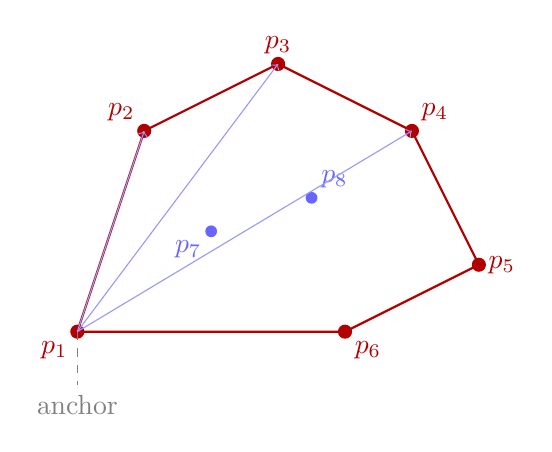
\begin{tikzpicture}[scale=0.85]
  \coordinate (p1) at (0,0);
  \coordinate (p2) at (1,3);
  \coordinate (p3) at (3,4);
  \coordinate (p4) at (5,3);
  \coordinate (p5) at (6,1);
  \coordinate (p6) at (4,0);
  \coordinate (p7) at (2,1.5);
  \coordinate (p8) at (3.5,2);
  \fill[blue!60] (p7) circle (2.5pt) node[below left] {$p_7$};
  \fill[blue!60] (p8) circle (2.5pt) node[above right] {$p_8$};
  \fill[red!70!black] (p1) circle (3pt) node[below left] {$p_1$};
  \fill[red!70!black] (p2) circle (3pt) node[above left] {$p_2$};
  \fill[red!70!black] (p3) circle (3pt) node[above] {$p_3$};
  \fill[red!70!black] (p4) circle (3pt) node[above right] {$p_4$};
  \fill[red!70!black] (p5) circle (3pt) node[right] {$p_5$};
  \fill[red!70!black] (p6) circle (3pt) node[below right] {$p_6$};
  \draw[thick,red!70!black] (p1)--(p2)--(p3)--(p4)--(p5)--(p6)--cycle;
  \draw[dashed,gray] (p1) -- ++(0,-0.8) node[below] {anchor};
  \draw[->,blue!40,thin] (p1) -- (p2);
  \draw[->,blue!40,thin] (p1) -- (p3);
  \draw[->,blue!40,thin] (p1) -- (p4);
\end{tikzpicture}
\caption{Graham Scan: the anchor point $p_1$ (lowest $y$) sorts all other points by polar angle. The hull vertices (red) are traced in counter-clockwise order.}
\label{fig:graham_scan}
\end{figure}


\subsection{Pseudocode}

\begin{algorithm}[htbp]
\caption{Graham Scan for Convex Hull}
\label{alg:graham_scan}
\begin{algorithmic}[1]
\Function{GrahamScan}{points}
  \If{$\text{len}(points) \le 2$}
    \State \Return $points$
  \EndIf
  \State $anchor \gets \min(points, \text{key}=\lambda p: (p.y, p.x))$
  \State $sorted\_points \gets \text{sorted}(points, \text{key}=\text{polar\_angle\_with\_anchor})$
  \State $hull \gets [\,]$
  \For{$p$ in $sorted\_points$}
    \While{$\text{len}(hull) \ge 2$ \textbf{and} $\text{cross\_product}(hull[-2], hull[-1], p) \le 0$}
      \State $hull.\text{pop}()$
    \EndWhile
    \State $hull.\text{append}(p)$
  \EndFor
  \State \Return $hull$
\EndFunction
\end{algorithmic}
\end{algorithm}

\subsection{Parameters}

\begin{itemize}
\item \textbf{Input}: A list of \texttt{Point2D} objects.
\item \textbf{Sorting Criterion}: Polar angle relative to the anchor. In the implementation, \texttt{math.atan2} is often used, but cross-products can provide a more robust (and sometimes faster) comparison.
\end{itemize}

\subsection{Complexity}

\begin{itemize}
\item \textbf{Time Complexity}: $O(n \log n)$\index{time complexity!$O(n \log n)$}, where $n$ is the number of points. This is dominated by the sorting step. The subsequent scan takes $O(n)$ time because each point is pushed and popped at most once.
\item \textbf{Space Complexity}: $O(n)$ to store the sorted points and the stack.
\end{itemize}

\begin{example}[Graham Scan Trace]\label{ex:graham_trace}
Consider the point set $P = \{(0,0),\, (1,1),\, (2,0),\, (1,-1),\, (0.5, 0.5)\}$.
\begin{enumerate}
\item The anchor point is $(0,0)$ (lowest $y$, then lowest $x$).
\item Sorting by polar angle around $(0,0)$ yields (approximately): $(1,-1),\, (2,0),\, (1,1),\, (0.5, 0.5)$.
\item The scan proceeds: $(0,0)$ and $(1,-1)$ are placed on the stack. When $(2,0)$ arrives, $\operatorname{cross}((0,0),(1,-1),(2,0)) = 1 \cdot 0 - (-1) \cdot 2 = 2 > 0$, so we keep the chain. When $(1,1)$ arrives, we check $\operatorname{cross}((1,-1),(2,0),(1,1)) = 1 \cdot 1 - 1 \cdot (-1) = 2 > 0$: no pop. When $(0.5, 0.5)$ arrives, $\operatorname{cross}((2,0),(1,1),(0.5,0.5)) = (-1)(0.5) - (1)(-1.5) = -0.5 + 1.5 = 1 > 0$: kept, but since $(0.5,0.5)$ lies in the interior of the hull formed by the other points, it will be interior to a final triangle and ultimately will not appear on the convex hull. (In practice, $(0.5,0.5)$ would be popped by a subsequent hull vertex check.)
\end{enumerate}
The resulting hull is $\{(0,0),\, (1,-1),\, (2,0),\, (1,1)\}$.
\end{example}

\subsection{Usages}

\begin{itemize}
\item Collision detection in physics engines.
\item Shape analysis and pattern recognition.
\item Geographic Information Systems (GIS) for defining boundary regions.
\item Minimum bounding box calculations.
\end{itemize}

\subsection{Testing and Edge Cases}

\begin{itemize}
\item \textbf{Few Points}: 0, 1, or 2 points should return the input points.
\item \textbf{Collinear Points}\index{collinear points}: Points lying on the same line. The algorithm should handle them by either including them or only keeping the endpoints (depending on the \texttt{cross\_product <= 0} vs \texttt{< 0} logic).
\item \textbf{Duplicate Points}\index{duplicate points}: Multiple points at the same coordinates.
\item \textbf{Degenerate Cases}: All points at the same location.
\item \textbf{Vertical/Horizontal alignment}: Points forming a perfect grid.
\end{itemize}

\subsection{References}

\begin{itemize}
\item Graham, R. L. (1972). ``An Efficient Algorithm for Determining the Convex Hull of a Finite Planar Set''. Information Processing Letters.
\item Cormen, T. H., Leiserson, C. E., Rivest, R. L., \& Stein, C. (2009). ``Introduction to Algorithms''. MIT Press.
\item Wikipedia: Graham scan.
\end{itemize}


\section{Monotone Chain}
\label{sec:monotone_chain}

The Monotone Chain algorithm (also known as Andrew's algorithm\index{Andrew's algorithm}) is a method for computing the convex hull of a finite set of points in the plane. It was first described by A.\ M.\ Andrew in 1979~\cite{andrew1979}. It is generally faster than the Graham scan because it avoids the calculation of polar angles and trigonometric functions, relying solely on sorting and cross-product tests.

\subsection{Definitions}

\begin{definition}[Upper and Lower Hull]\label{def:upper_lower_hull}
Let $P$ be a set of points sorted lexicographically. The \emph{lower hull} is the sequence of vertices of $\operatorname{conv}(P)$ from the leftmost to the rightmost point, traversed along the bottom boundary. The \emph{upper hull} is the analogous sequence traversed along the top boundary. Together they partition the hull boundary into two monotone chains.
\end{definition}

\begin{definition}[Orientation Test]\label{def:orientation_test}
The \emph{orientation test}\index{orientation test} for three points $A, B, C \in \mathbb{R}^2$ computes the sign of $\operatorname{cross}(A, B, C)$. It determines whether the path $A \to B \to C$ makes a left turn, right turn, or is collinear.
\end{definition}

\subsection{Theory}

The algorithm takes advantage of the fact that the convex hull can be split into upper and lower chains. By sorting the points lexicographically (first by $x$-coordinate, then by $y$-coordinate), we can build the lower hull by scanning the sorted points from left to right. A similar process (scanning either the reversed points or right-to-left) yields the upper hull. For each chain, the algorithm maintains a stack and removes the last point if it doesn't form a ``valid'' turn relative to the previous points.

\begin{theorem}[Correctness of Monotone Chain]\label{thm:monotone_chain_correctness}
Let $P$ be a set of $n \ge 2$ points in $\mathbb{R}^2$. After sorting $P$ lexicographically, the Monotone Chain algorithm correctly computes $\operatorname{conv}(P)$.
\end{theorem}
\begin{proof}
The sorted order ensures the lower hull is built left-to-right with monotonically increasing $x$-coordinates. At each step, the invariant is that the stack maintains a chain with all cross products positive (left turns). If adding a point $p$ would create a non-positive cross product with the last two stack points, the middle point cannot be a vertex of the convex hull (it is ``inside'' the angle formed by the other two). Removing it preserves the invariant. The upper hull is built symmetrically. The concatenation of lower and upper hulls (with endpoints removed to avoid duplication) gives the full convex hull boundary.
\end{proof}

\subsection{Pseudocode}

\begin{algorithm}[htbp]
\caption{Monotone Chain (Andrew's Algorithm)}
\label{alg:monotone_chain}
\begin{algorithmic}[1]
\Function{MonotoneChain}{points}
  \If{$\text{len}(points) \le 2$}
    \State \Return $points$
  \EndIf
  \State $points.\text{sort}()$
  \State $lower \gets [\,]$
  \For{$p$ in $points$}
    \While{$\text{len}(lower) \ge 2$ \textbf{and} $\text{cross\_product}(lower[-2], lower[-1], p) \le 0$}
      \State $lower.\text{pop}()$
    \EndWhile
    \State $lower.\text{append}(p)$
  \EndFor
  \State $upper \gets [\,]$
  \For{$p$ in $\text{reversed}(points)$}
    \While{$\text{len}(upper) \ge 2$ \textbf{and} $\text{cross\_product}(upper[-2], upper[-1], p) \le 0$}
      \State $upper.\text{pop}()$
    \EndWhile
    \State $upper.\text{append}(p)$
  \EndFor
  \State \Return $lower[:-1] + upper[:-1]$
\EndFunction
\end{algorithmic}
\end{algorithm}

\subsection{Parameters}

\begin{itemize}
\item \textbf{Input}: A list of \texttt{Point2D} objects.
\item \textbf{Sorting Key}: Points are sorted primarily by their $x$-coordinate and secondarily by their $y$-coordinate.
\end{itemize}

\subsection{Complexity}

\begin{itemize}
\item \textbf{Time Complexity}: $O(n \log n)$ due to sorting. The construction phase is strictly $O(n)$, as each point is added and removed at most once for each hull.
\item \textbf{Space Complexity}: $O(n)$ to hold the sorted points and the resulting hull.
\end{itemize}

\subsection{Usages}

\begin{itemize}
\item Standard 2D convex hull calculation in many libraries (e.g., SciPy as a fallback).
\item Calculating the area of a set of points.
\item Simplifying complex polygons.
\item GIS and map boundary creation.
\end{itemize}

\subsection{Testing and Edge Cases}

\begin{itemize}
\item \textbf{Vertical Lines}: Points with the same $x$-coordinate but different $y$-coordinates.
\item \textbf{Collinear Points}: Handled by the \texttt{>= 2} and \texttt{cross\_product <= 0} conditions.
\item \textbf{Identical Points}: Lexicographical sort handles duplicates naturally.
\item \textbf{Small Sets}: Sets of 0, 1, or 2 points return early.
\item \textbf{Closed Hulls}: Ensure the first point and last point of each chain match up correctly at the extremities.
\end{itemize}

\subsection{References}

\begin{itemize}
\item Andrew, A. M. (1979). ``Another Efficient Algorithm for Convex Hulls in Two Dimensions''. Information Processing Letters.
\item Preparata, F. P., \& Shamos, M. I. (1985). ``Computational Geometry: An Introduction''. Springer-Verlag.
\item Wikipedia: Monotone chain.
\end{itemize}


\section{Chan's Algorithm}
\label{sec:chans_algorithm}

Chan's algorithm is an \textbf{output-sensitive}\index{output-sensitive algorithm} algorithm for computing the convex hull of a set of $n$ points in 2D or 3D. It combines the strengths of Graham scan (or \cref{alg:monotone_chain}) and Jarvis march to achieve an optimal $O(n \log h)$ running time, where $h$ is the number of vertices on the convex hull. It was introduced by Chan in 1996~\cite{chan1996}.

\subsection{Definitions}

\begin{definition}[Output-Sensitive Algorithm]\label{def:output_sensitive}
An algorithm is \emph{output-sensitive} if its running time depends not only on the input size $n$ but also on the output size (in this case, $h$, the number of hull vertices).
\end{definition}

\subsection{Theory}

Chan's algorithm partitions the point set into $n/m$ groups of size $m$. It computes the convex hull of each group in $O(m \log m)$ time. Then, it uses a modified Jarvis march to find the global hull by performing binary searches (tangent queries) on the mini-hulls. By iteratively guessing $m = 2^{2^t}$, it reaches the optimal complexity.

\begin{theorem}[Complexity of Chan's Algorithm]\label{thm:chans_complexity}
Chan's algorithm computes the convex hull of $n$ points in $O(n \log h)$ time and $O(n)$ space, where $h$ is the number of vertices on the convex hull.
\end{theorem}
\begin{proof}
The algorithm tries group sizes $m = 2, 4, 16, 256, \ldots, 2^{2^t}$. For the correct guess where $m \ge h$, each group hull is computed in $O(m \log m)$ time, and the Jarvis march finds the hull in $O(m \log m)$ tangent queries (each taking $O(\log m)$ time on a group hull of size $\le m$). The total work is $O((n/m) \cdot m \log m) = O(n \log m) = O(n \log h)$. All previous incorrect guesses $m' < h$ contribute at most $\sum_{t} O(n \log 2^{2^t}) = O(n)$ total work by a geometric series argument.
\end{proof}

\subsection{Pseudocode}

\begin{algorithm}[htbp]
\caption{Chan's Convex Hull Algorithm}
\label{alg:chans_hull}
\begin{algorithmic}[1]
\Function{ChansConvexHull}{$P$}
  \For{$t = 1, 2, \ldots$}
    \State $m \gets \min(2^{2^t}, n)$
    \State Partition $P$ into groups of size $m$
    \State Compute Monotone Chain hull for each group
    \State \Comment{Try to find global hull using Jarvis march in $m$ steps}
    \State From current point, find next hull point by tangent query on each mini-hull
    \If{hull is closed}
      \State \Return hull
    \EndIf
  \EndFor
\EndFunction
\end{algorithmic}
\end{algorithm}

\subsection{Parameters}

\begin{itemize}
\item \textbf{Group Size ($m$)}: Controlled by the iteration parameter $t$.
\end{itemize}

\subsection{Complexity}

\begin{itemize}
\item \textbf{Time}: $O(n \log h)$\index{time complexity!$O(n \log h)$}, which is optimal.
\item \textbf{Space}: $O(n)$.
\end{itemize}

\subsection{Usages}

Implemented in \texttt{compgeom.polygon.convex\_hull.Chan}. Used for efficient hull calculation when the number of hull vertices is small.

\subsection{Testing and Edge Cases}

\begin{itemize}
\item \textbf{Testing}: Compare output with Graham Scan or SciPy's Qhull. Verify all original points are inside the hull.
\item \textbf{Edge Cases}: Collinear points, coincident points, small point sets ($n < 3$).
\end{itemize}

\subsection{References}

\begin{itemize}
\item Chan, T. M. (1996). ``Optimal output-sensitive convex hull algorithms in two and three dimensions''. Discrete \& Computational Geometry.
\item Wikipedia: Chan's algorithm.
\end{itemize}


\section{QuickHull}
\label{sec:quickhull}

QuickHull is a divide-and-conquer\index{divide and conquer} algorithm for computing the convex hull of a finite set of points. It is similar in design to the Quicksort sorting algorithm. It was independently published by several researchers, including Barber et al.\ (1996)~\cite{barber1996} and Eddy (1977)~\cite{eddy1977}, and is the basis of the widely used \texttt{Qhull} library.

\subsection{Definitions}

\begin{definition}[Distance from a Line]\label{def:dist_from_line}
The \emph{perpendicular distance} from a point $P$ to a line through points $A$ and $B$ is
\[
d(P, \overline{AB}) = \frac{|\operatorname{cross}(A, B, P)|}{\|B - A\|}.
\]
Points farthest from a line segment are guaranteed to be vertices of the convex hull.
\end{definition}

\subsection{Theory}

The algorithm begins by finding the leftmost and rightmost points, which are guaranteed to be on the hull. These points divide the point set into two subsets by a line. For each subset, the point farthest from the line is identified. This point, along with the two original points, forms a triangle. Points inside this triangle cannot be on the convex hull and are discarded. The process is then recursively applied to the two edges of the triangle that are not part of the original line.

\begin{theorem}[QuickHull Average-Case Complexity]\label{thm:quickhull_avg}
The average-case time complexity of QuickHull is $O(n \log n)$ when points are distributed according to a smooth distribution (e.g., uniformly in a convex region).
\end{theorem}
\begin{proof}
The argument mirrors that of Quicksort. On average, the farthest point partitions the remaining points into two roughly balanced subsets. If each recursive step discards a constant fraction of the remaining points, the depth of recursion is $O(\log n)$ and the total work is $O(n \log n)$. In the worst case (e.g., points on a circle), the partition is maximally unbalanced and the complexity degrades to $O(n^2)$.
\end{proof}

\subsection{Pseudocode}

\begin{algorithm}[htbp]
\caption{QuickHull Algorithm}
\label{alg:quickhull}
\begin{algorithmic}[1]
\Function{QuickHull}{points}
  \State $leftmost \gets \min(points)$
  \State $rightmost \gets \max(points)$
  \State $upper \gets$ points above line $(leftmost, rightmost)$
  \State $lower \gets$ points below line $(leftmost, rightmost)$
  \State \Return $[leftmost] + \text{FindHull}(leftmost, rightmost, upper) + [rightmost] + \text{FindHull}(rightmost, leftmost, lower)$
\EndFunction

\Function{FindHull}{$A, B$, candidates}
  \If{candidates is empty}
    \State \Return $[\,]$
  \EndIf
  \State $P \gets \arg\max_{p \in \text{candidates}} \text{dist\_from\_line}(A, B, p)$
  \State $left\_of\_AP \gets [p \mid p \in \text{candidates} \wedge \text{is\_left\_of}(A, P, p)]$
  \State $left\_of\_PB \gets [p \mid p \in \text{candidates} \wedge \text{is\_left\_of}(P, B, p)]$
  \State \Return $\text{FindHull}(A, P, left\_of\_AP) + [P] + \text{FindHull}(P, B, left\_of\_PB)$
\EndFunction
\end{algorithmic}
\end{algorithm}

\subsection{Parameters}

\begin{itemize}
\item \textbf{Input}: A set of points (list of \texttt{Point2D}).
\item \textbf{Recursive termination}: When the subset of candidate points for a segment is empty.
\end{itemize}

\subsection{Complexity}

\begin{itemize}
\item \textbf{Time Complexity}: Average case $O(n \log n)$. Worst case $O(n^2)$\index{time complexity!$O(n^2)$} when points are distributed such that the partition is highly unbalanced (e.g., points on a circle).
\item \textbf{Space Complexity}: $O(n)$ to store the points and recursion stack.
\end{itemize}

\subsection{Usages}

\begin{itemize}
\item The primary algorithm in the \texttt{Qhull} library, used by SciPy, MATLAB, and R.
\item General-purpose convex hull calculation in 2D and 3D.
\item Collision detection and mesh simplification.
\end{itemize}

\subsection{Testing and Edge Cases}

\begin{itemize}
\item \textbf{Highly Symmetric Points}: Points on a circle can lead to the worst-case $O(n^2)$ performance.
\item \textbf{Collinear Points}: Farthest point might not be unique; handle tie-breaking consistently.
\item \textbf{Points inside the hull}: Ensure that the pruning (ignoring points inside triangles) is correct.
\item \textbf{Numerical Precision}: Use an epsilon for distance and cross-product comparisons to avoid issues with floating-point arithmetic.
\end{itemize}

\subsection{References}

\begin{itemize}
\item Barber, C. B., Dobkin, D. P., \& Huhdanpaa, H. (1996). ``The Quickhull Algorithm for Convex Hulls''. ACM Transactions on Mathematical Software (TOMS).
\item Eddy, W. F. (1977). ``A New Convex Hull Algorithm for Planar Sets''. ACM Transactions on Mathematical Software (TOMS).
\item Bykat, A. (1978). ``Convex Hull of a Finite Set of Points in Two Dimensions''. Information Processing Letters.
\item Wikipedia: Quickhull.
\end{itemize}


\section{Convex Hull Peeling}
\label{sec:convex_hull_peeling}

Convex hull peeling\index{convex hull peeling}, also known as ``onion peeling''\index{onion peeling}, is a recursive process of identifying and removing the convex hull of a point set. After the first hull is removed, the process is repeated on the remaining points until no points are left. This decomposition organizes a set of points into nested ``layers,'' similar to the layers of an onion. It was studied by Chazelle~\cite{chazelle1985}, Overmars and van Leeuwen~\cite{overmars1981}, and is closely related to the concept of Tukey depth introduced by Tukey~\cite{tukey1975}. It is a fundamental technique for robust statistics, data depth analysis, and identifying outliers.

\subsection{Definitions}

\begin{definition}[Convex Hull Layer]\label{def:hull_layer}
A \emph{convex hull layer} is the set of points forming the boundary of the convex hull at a specific iteration of the peeling process.
\end{definition}

\begin{definition}[Convex Hull Depth]\label{def:hull_depth}
The \emph{convex hull depth} (or layer number) of a point is the iteration number at which it is removed. Points on the outermost hull have depth~1. The innermost layer defines the \textbf{Tukey depth}\index{Tukey depth} of the deepest points.
\end{definition}

\subsection{Theory}

The onion peeling of a point set $P$ provides a natural way to measure the ``centrality'' of points.
\begin{enumerate}
\item Compute the convex hull $CH(P)$.
\item The points on the boundary of $CH(P)$ form the first layer $L_1$.
\item Let $P' = P \setminus L_1$.
\item Repeat the process on $P'$ to find $L_2, L_3, \dots, L_k$.
\end{enumerate}

\begin{theorem}[Layer Count]\label{thm:layer_count}
For $n$ points distributed uniformly at random in a unit square, the expected number of layers is $\Theta(n^{2/3})$.
\end{theorem}
\begin{proof}
Each convex hull of a random point set in the unit square has $O(n^{1/3})$ vertices on average. Removing these vertices reduces the remaining set by this amount. The number of layers before the set is exhausted is thus $O(n / n^{1/3}) = O(n^{2/3})$. A matching lower bound follows from concentration arguments on the extreme point count.
\end{proof}

In 2D, the total number of layers $k$ is roughly $O(n^{2/3})$ for points distributed uniformly in a square. The structure of the layers can be used to define the Tukey Depth of points in a multivariate dataset.

\begin{figure}[htbp]
\centering
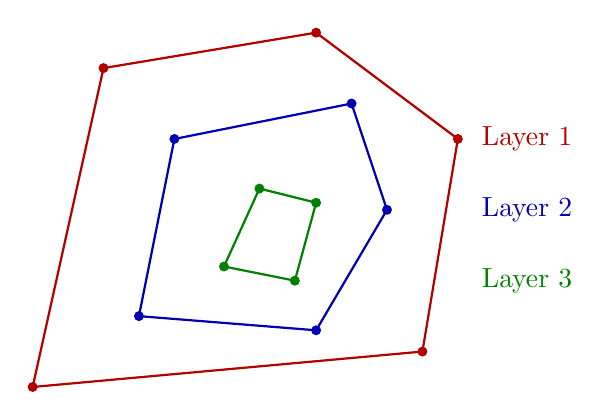
\begin{tikzpicture}[scale=0.9]
  \draw[thick,red!70!black] (-3,-2)--(-2,2.5)--(1,3)--(3,1.5)--(2.5,-1.5)--cycle;
  \node[red!70!black,right] at (3.2,1.5) {Layer 1};
  \draw[thick,blue!70!black] (-1.5,-1)--(-1,1.5)--(1.5,2)--(2,0.5)--(1,-1.2)--cycle;
  \node[blue!70!black,right] at (3.2,0.5) {Layer 2};
  \draw[thick,green!50!black] (-0.3,-0.3)--(0.2,0.8)--(1,0.6)--(0.7,-0.5)--cycle;
  \node[green!50!black,right] at (3.2,-0.5) {Layer 3};
  \foreach \p in {(-3,-2),(-2,2.5),(1,3),(3,1.5),(2.5,-1.5)} {\fill[red!70!black] \p circle (2pt);}
  \foreach \p in {(-1.5,-1),(-1,1.5),(1.5,2),(2,0.5),(1,-1.2)} {\fill[blue!70!black] \p circle (2pt);}
  \foreach \p in {(-0.3,-0.3),(0.2,0.8),(1,0.6),(0.7,-0.5)} {\fill[green!50!black] \p circle (2pt);}
\end{tikzpicture}
\caption{Convex hull peeling (onion peeling): successive convex hulls are removed, producing nested layers.}
\label{fig:onion_peeling}
\end{figure}


\subsection{Pseudocode}

\begin{algorithm}[htbp]
\caption{Convex Hull Peeling (Onion Peeling)}
\label{alg:onion_peeling}
\begin{algorithmic}[1]
\Function{ConvexHullPeeling}{points}
  \State $layers \gets [\,]$
  \State $current\_points \gets \text{set}(points)$
  \While{$current\_points$ is not empty}
    \If{$\text{len}(current\_points) < 3$}
      \State $layers.\text{append}(\text{list}(current\_points))$
      \State \textbf{break}
    \EndIf
    \State $hull\_indices \gets \text{ComputeConvexHull}(\text{list}(current\_points))$
    \State $hull\_points \gets [\text{list}(current\_points)[i] \mid i \in hull\_indices]$
    \State $layers.\text{append}(hull\_points)$
    \For{$p$ in $hull\_points$}
      \State $current\_points.\text{remove}(p)$
    \EndFor
  \EndWhile
  \State \Return $layers$
\EndFunction
\end{algorithmic}
\end{algorithm}

\subsection{Parameters}

\begin{itemize}
\item \textbf{Hull Algorithm}: Monotone Chain or Graham Scan are ideal for 2D. For 3D, QuickHull is standard.
\item \textbf{Handling Collinearity}: Points that lie exactly on the edges of the convex hull can either be included in the current layer or treated as interior points for the next layer. Including them is more common in statistics.
\end{itemize}

\subsection{Complexity}

\begin{itemize}
\item \textbf{Naive Complexity}: $O(n^2)$\index{time complexity!$O(n^2)$} if a new $O(n \log n)$ hull is calculated for every point removed.
\item \textbf{Efficient 2D Complexity}: $O(n \log n)$ using Chazelle's algorithm~\cite{chazelle1985}, which uses a more complex data structure to update the hull as points are removed.
\item \textbf{Space Complexity}: $O(n)$ to store the point set and the layer indices.
\end{itemize}

\subsection{Usages}

\begin{itemize}
\item \textbf{Robust Statistics}: Identifying the ``geometric median'' of a point set by finding the deepest onion layer.
\item \textbf{Outlier Detection}\index{outlier detection}: Points in the first few layers are candidates for being outliers or ``extreme'' values.
\item \textbf{Data Visualization}: Creating ``bagplots'' or ``boxplots'' for 2D data.
\item \textbf{Pattern Recognition}: Describing the density and distribution of a point cloud.
\item \textbf{Computational Geometry}: A preprocessing step for certain range-searching and visibility problems.
\end{itemize}

\begin{example}[Onion Peeling by Hand]\label{ex:onion_peeling}
Consider a $3 \times 3$ grid of points $P = \{(i,j) : i,j \in \{0,1,2\}\}$ with 9 total points.
\begin{enumerate}
\item Layer 1 (outermost hull): The 8 boundary points $\{(0,0),(1,0),(2,0),(2,1),(2,2),(1,2),(0,2),(0,1)\}$.
\item After peeling, only $\{(1,1)\}$ remains.
\item Layer 2: The single point $\{(1,1)\}$.
\end{enumerate}
The center point has hull depth~2, while all other points have depth~1.
\end{example}

\subsection{Testing and Edge Cases}

\begin{itemize}
\item \textbf{Perfectly Collinear Points}: All points should be removed in the first layer.
\item \textbf{Points on a Circle}: All points should be removed in the first layer.
\item \textbf{Grid Arrangement}: Verify that the peeling correctly identifies the nested squares or rectangles.
\item \textbf{Small Sets}: Test with $n=1, 2, 3$.
\item \textbf{Symmetry}: For a symmetric distribution, the layers should maintain that symmetry.
\end{itemize}

\subsection{References}

\begin{itemize}
\item Chazelle, B. (1985). ``On the convex layers of a planar set''. IEEE Transactions on Information Theory.
\item Overmars, M. H., \& Leeuwen, J. van. (1981). ``Maintenance of configurations in the plane''. Journal of Computer and System Sciences.
\item Tukey, J. W. (1975). ``Mathematics and the picturing of data''. Proceedings of the International Congress of Mathematicians.
\item Wikipedia: Convex layers.
\end{itemize}


